\chapter{Métodos}
\label{metodos}

Este capítulo describe la metodología empleada en el desarrollo del sistema de aprendizaje de idiomas, incluyendo la arquitectura del sistema, la implementación de los componentes, los algoritmos desarrollados y la metodología de evaluación.

\section{Arquitectura del Sistema}
\label{arquitectura-sistema}

El sistema se ha diseñado siguiendo una arquitectura modular y escalable que integra tecnologías de vanguardia en \gls{ia} y procesamiento de lenguaje natural. La arquitectura se divide en dos componentes principales: frontend y backend, comunicados a través de una API REST.

\begin{figure}[H]
  \centering
  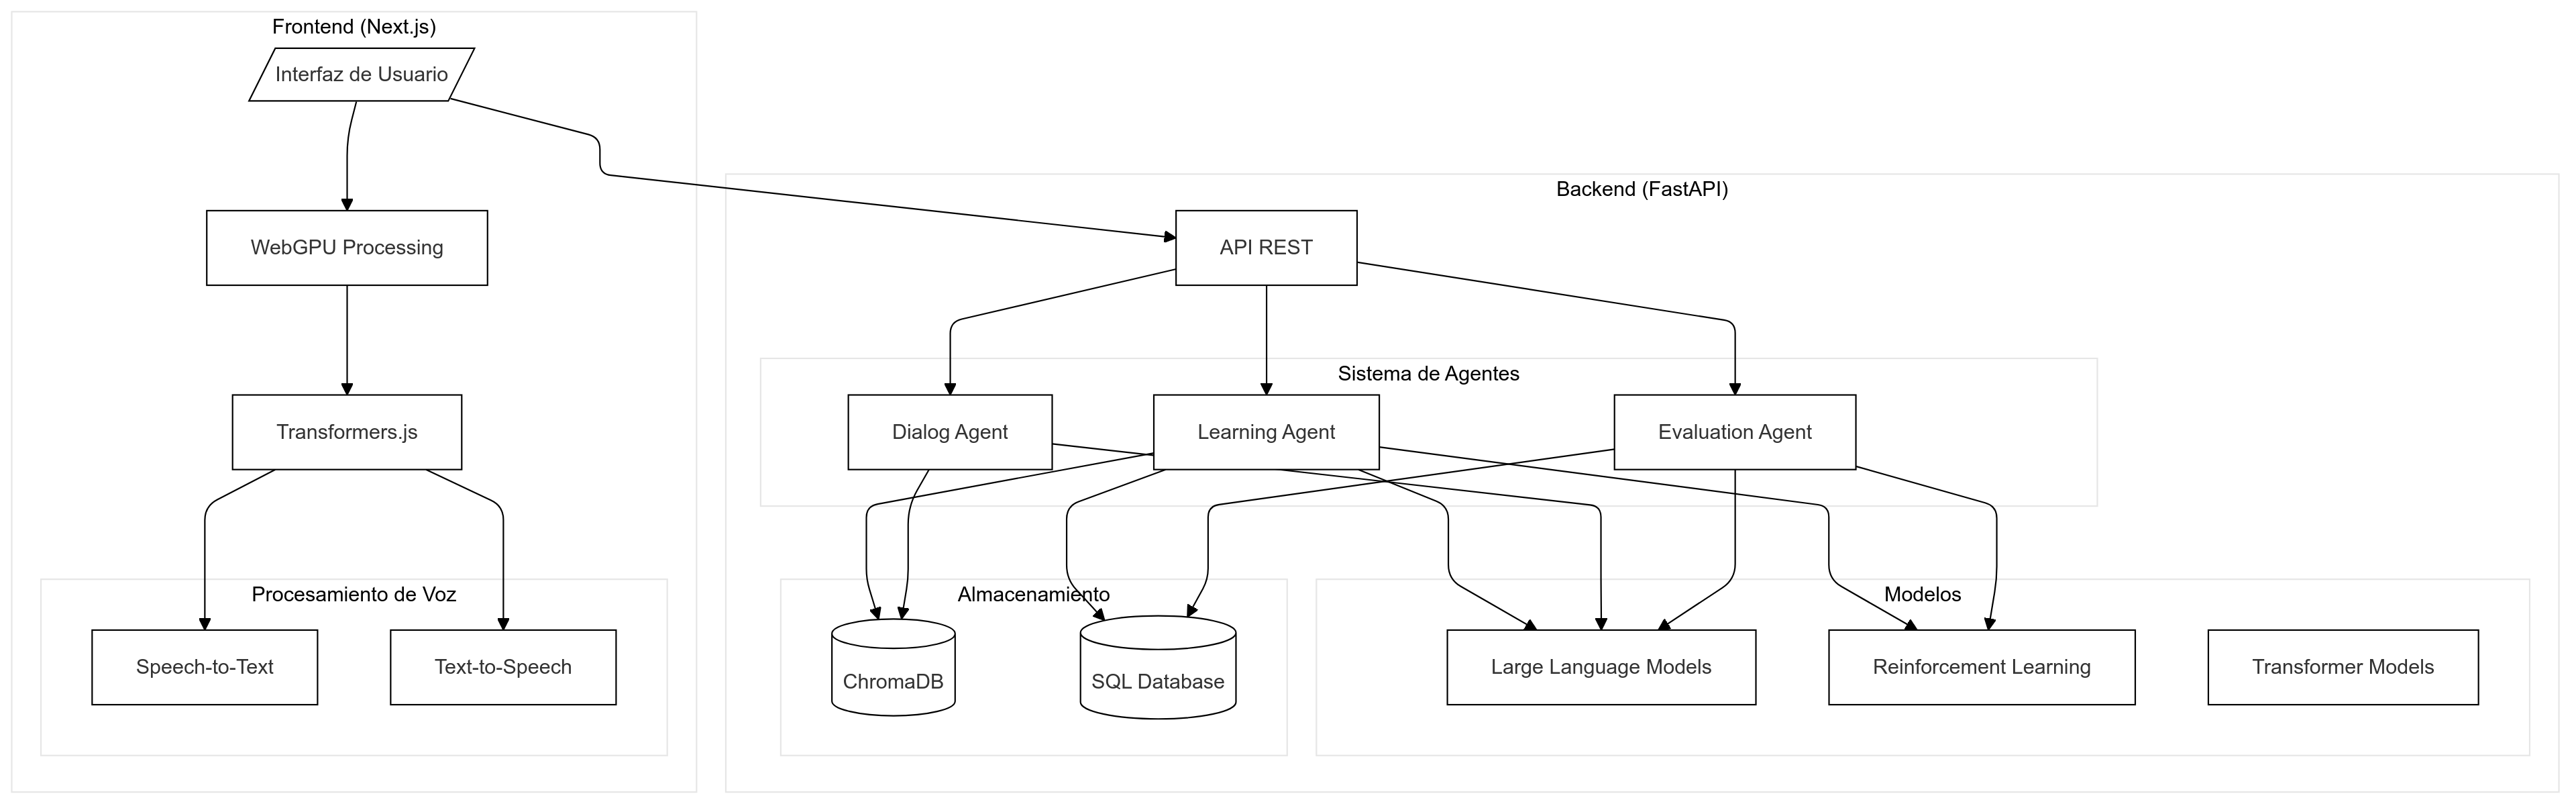
\includegraphics[width=0.8\textwidth]{figuras/architecture.png}
    \caption{Arquitectura del Sistema}
    \label{fig:arquitectura-sistema}
    % Aquí se insertará el diagrama Mermaid generado
\end{figure}


\subsection{Frontend}
\label{frontend}

El frontend del sistema se implementa utilizando Next.js y está basado en el framework \gls{assistant-ui}, un proyecto \gls{open-source} que facilita la integración de interfaces de chat con LangGraph. Esta decisión arquitectónica permite una rápida implementación de funcionalidades de chat mientras mantiene la flexibilidad para personalizaciones específicas del dominio.

\begin{figure}[H]
    \centering
    \caption{Arquitectura del Frontend}
    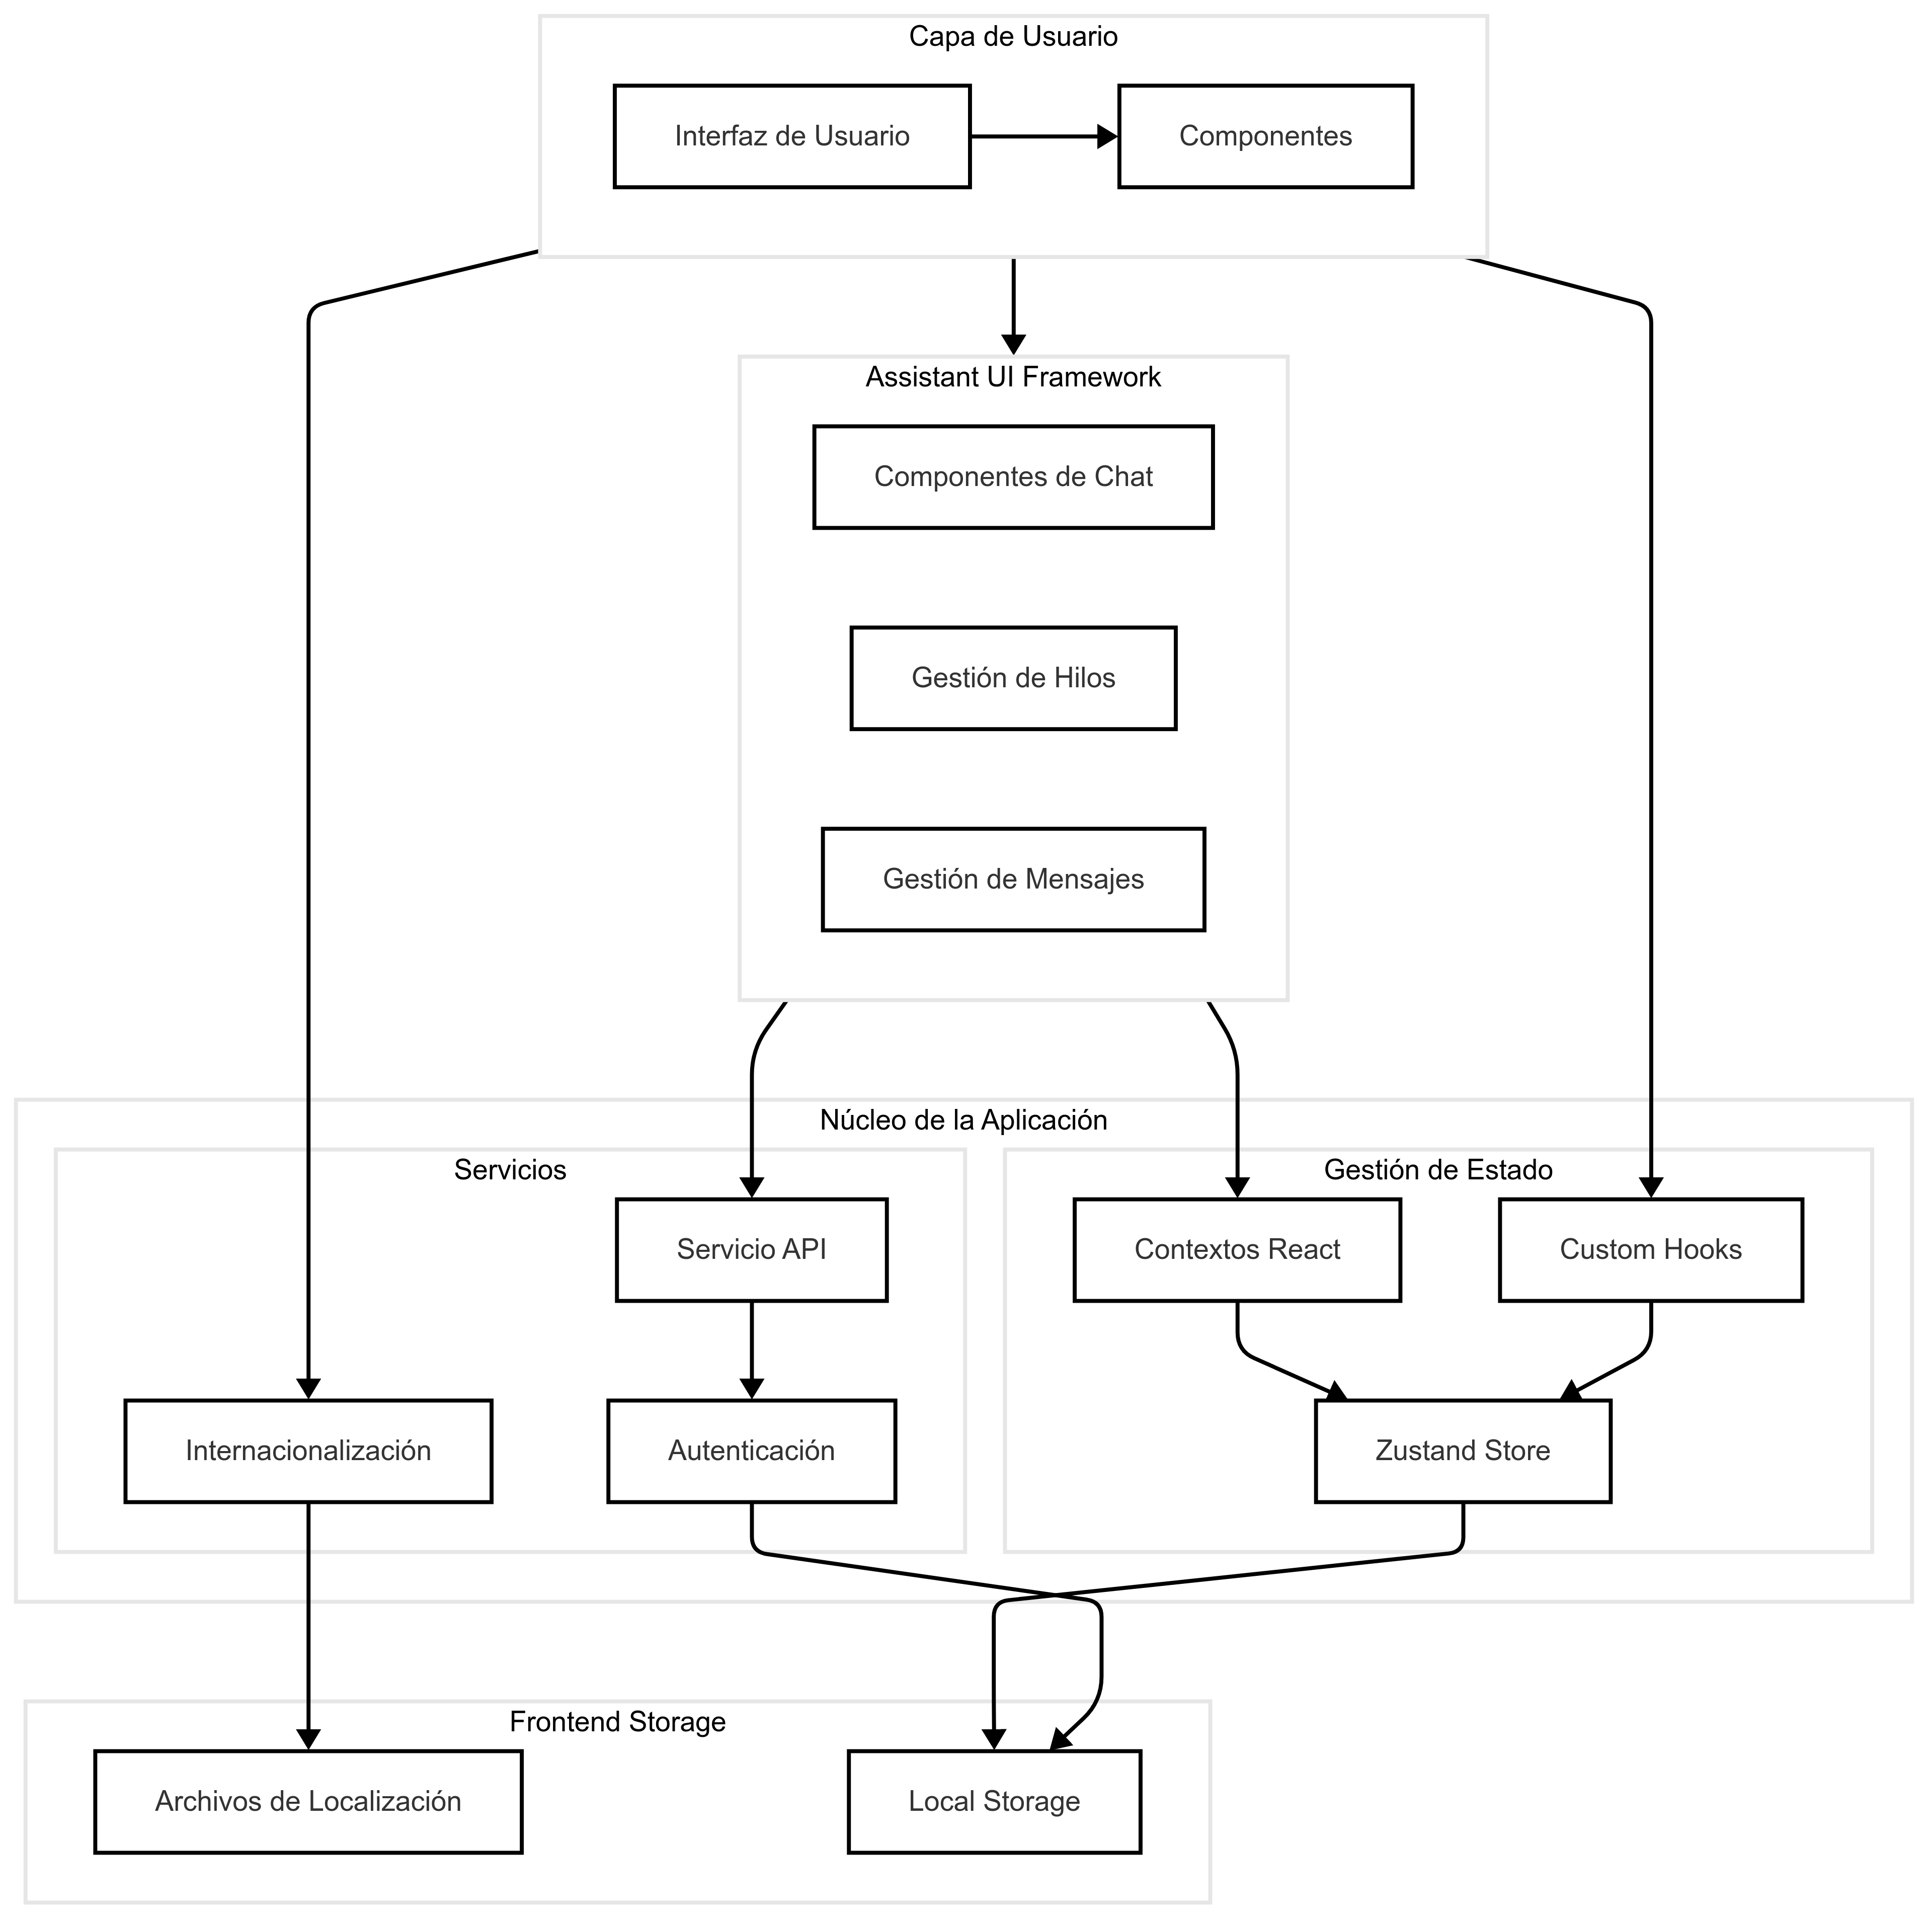
\includegraphics[width=0.8\textwidth]{figuras/frontend.png}
    \label{fig:arquitectura-frontend}
    % Aquí se insertará el diagrama Mermaid generado
\end{figure}

\subsubsection{Assistant UI Framework}
\label{assistant-ui}

El sistema se construye sobre \gls{assistant-ui}, que proporciona:

\begin{itemize}
    \item \textbf{Componentes de Chat}:
    \begin{itemize}
        \item Interfaz de chat prediseñada y personalizable
        \item Sistema de renderizado de mensajes
        \item Gestión de entrada de usuario
    \end{itemize}

    \item \textbf{Gestión de Hilos}:
    \begin{itemize}
        \item Sistema de hilos de conversación
        \item Persistencia de contexto conversacional
        \item Manejo de múltiples conversaciones
    \end{itemize}

    \item \textbf{Integración con LangGraph}:
    \begin{itemize}
        \item Conexión directa con el backend de LangGraph
        \item Gestión de estados de agentes
        \item Sistema de eventos para actualizaciones en tiempo real
    \end{itemize}
\end{itemize}

\subsubsection{Arquitectura de Componentes}
La arquitectura del frontend se organiza en las siguientes capas:

\begin{itemize}
    \item \textbf{Capa de Usuario}:
    \begin{itemize}
        \item Implementación de páginas y rutas utilizando el sistema de enrutamiento de Next.js
        \item Componentes reutilizables para interfaz de usuario
        \item Implementación de layouts y templates adaptables
    \end{itemize}

    \item \textbf{Núcleo de la Aplicación}:
    \begin{itemize}
        \item Gestión de estado utilizando Context API y custom hooks
        \item Servicios para comunicación con el backend
        \item Motor de procesamiento de voz
    \end{itemize}

    \item \textbf{Utilidades}:
    \begin{itemize}
        \item Funciones de validación y formateo
        \item Manejadores de errores globales
        \item Helpers para formateo y transformación de datos
    \end{itemize}
\end{itemize}


\subsubsection{Servicios de Comunicación}
\label{servicios-comunicacion}

La comunicación con el backend se gestiona a través de servicios especializados:

\begin{itemize}
    \item \textbf{API Service}:
    \begin{itemize}
        \item Implementación de cliente HTTP basado en Axios
        \item Sistema de interceptores para manejo de errores
        \item Caché de respuestas para optimización de rendimiento
        \item Integración con endpoints de LangGraph
    \end{itemize}

    \item \textbf{Gestión de Autenticación}:
    \begin{itemize}
        \item Sistema de autenticación basado en tokens
        \item Manejo de sesiones de usuario
        \item Protección de rutas y recursos
    \end{itemize}
\end{itemize}

\subsection{Backend}
\label{backend}

El backend del sistema se implementa utilizando FastAPI como framework principal, incorporando un sistema multi-agente basado en LangGraph para la gestión de la lógica de aprendizaje. La arquitectura se organiza en capas claramente definidas que gestionan diferentes aspectos del sistema.

\begin{figure}[H]
    \centering
    \caption{Arquitectura del Backend}
    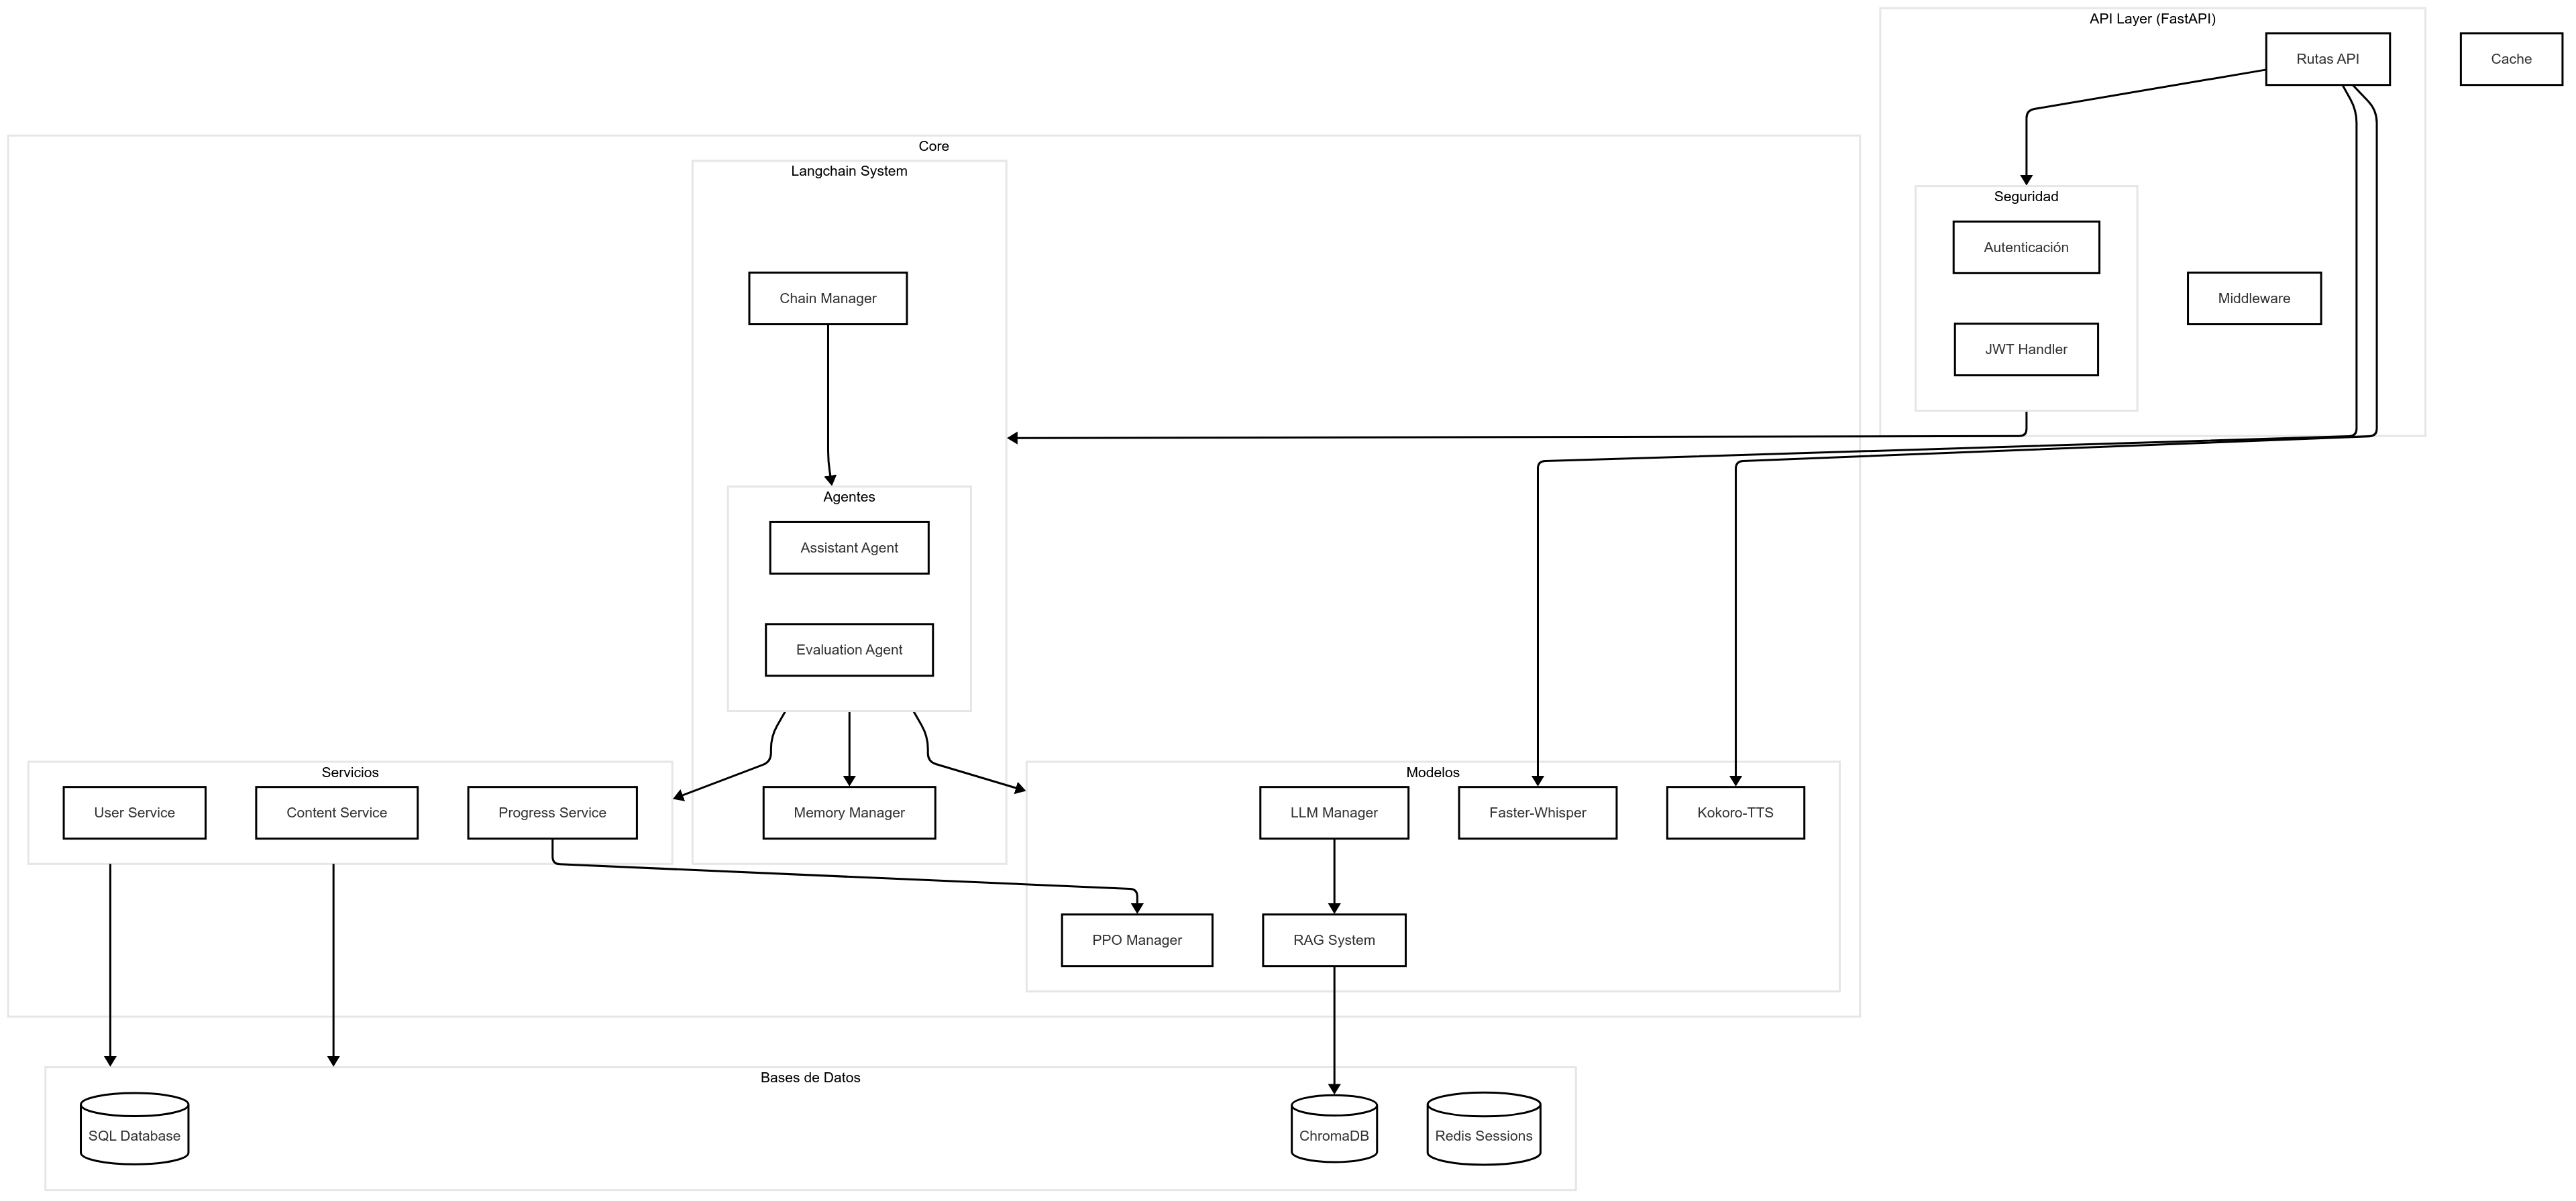
\includegraphics[width=0.8\textwidth]{figuras/backend.png}
    \label{fig:arquitectura-backend}
\end{figure}

  

\subsubsection{Capa de API}
\label{capa-api}

La capa de API, implementada con FastAPI, gestiona todas las interacciones con el cliente a través de endpoints RESTful. El sistema proporciona documentación automática mediante OpenAPI y realiza validación de datos utilizando Pydantic. La seguridad se maneja a través de middleware específico que incluye autenticación JWT, rate limiting para prevención de abusos y un sistema de validación de permisos basado en roles. Adicionalmente, se implementa CORS para seguridad entre dominios y un sistema de logging para el monitoreo de solicitudes.

\subsubsection{Sistema Multi-Agente}
\label{sistema-multi-agente}

El corazón del sistema es la implementación multi-agente utilizando LangGraph, que consta de tres agentes especializados. El Learning Agent se encarga de gestionar las rutas de aprendizaje personalizadas y la adaptación dinámica del contenido, implementando algoritmos de \gls{rl}. El Dialog Agent maneja las conversaciones con el usuario, integrándose con modelos \gls{llm} y utilizando un sistema de \gls{rag} para contextualización. Por su parte, el Evaluation Agent realiza la evaluación continua del progreso, analiza patrones de error y ajusta los parámetros de aprendizaje según sea necesario.

\subsubsection{Gestión de Modelos}
\label{gestion-modelos}

La integración de modelos de \gls{ia} se realiza a través de gestores especializados. El LLM Manager coordina la integración con modelos de lenguaje, gestionando prompts, contextos y optimizando recursos computacionales. El RL Manager implementa algoritmos \gls{ppo}, manejando estados y recompensas para optimizar las políticas de aprendizaje. El sistema RAG se encarga de la indexación de contenido educativo, realizando búsquedas semánticas mediante ChromaDB y generando respuestas contextualizadas.

\subsubsection{Servicios Core}
\label{servicios-core}

Los servicios principales del sistema se dividen en tres componentes fundamentales. Primero, el User Service, que gestiona los perfiles de usuario, preferencias y análisis de comportamiento. Segundo, el Content Service, encargado de la gestión, adaptación y versionado de recursos educativos. Tercero, el Progress Service, que realiza el seguimiento del avance de los estudiantes, genera reportes y analiza métricas de rendimiento.

\subsubsection{Capa de Datos}
\label{capa-datos}

La gestión de datos se implementa mediante un sistema dual de almacenamiento. La base de datos SQL se utiliza para datos estructurados y relaciones entre entidades, con optimización de consultas para máximo rendimiento. ChromaDB, como base de datos vectorial, maneja el almacenamiento de embeddings y permite realizar búsquedas semánticas eficientes. Complementariamente, se utiliza Redis como sistema de caché para optimizar el acceso a datos frecuentes, gestionar sesiones y almacenar estados temporales.

\subsubsection{Optimización y Monitoreo}
\label{optimizacion-monitoreo}

El sistema implementa estrategias integrales para garantizar rendimiento y fiabilidad. El monitoreo se realiza mediante logging estructurado de eventos y métricas de rendimiento, con un sistema de alertas automáticas. La optimización incluye implementación de caché en múltiples niveles, pooling de conexiones y balanceo de carga. La escalabilidad se asegura mediante una arquitectura stateless, containerización con Docker y un sistema de configuración distribuida.


\section{Implementación de los Componentes}
\label{implementacion-componentes}

Esta sección detalla la implementación técnica de los componentes principales del sistema: el sistema de agentes y el procesamiento de voz. Cada componente se ha desarrollado considerando los requisitos de rendimiento, escalabilidad y usabilidad del sistema.

\subsection{Sistema de Agentes}
\label{implementacion-agentes}

El sistema implementa tres agentes especializados utilizando LangGraph como framework base. Cada agente está diseñado con responsabilidades específicas y se comunica con los demás a través de un sistema de mensajería asíncrona.

El Learning Agent se implementa como un agente basado en políticas de \gls{rl}. Utiliza el algoritmo \gls{ppo} para optimizar las decisiones de contenido y rutas de aprendizaje. El agente mantiene un estado que incluye el perfil del estudiante, su historial de aprendizaje y sus objetivos. Para la selección de contenido, implementa un sistema de ranking que considera múltiples factores como dificultad, relevancia y preferencias del usuario.

El Dialog Agent se construye sobre un modelo \gls{llm} con un sistema de \gls{rag} para contextualización. El agente implementa un gestor de estado de diálogo que mantiene el contexto de la conversación y coordina las respuestas. Para garantizar la coherencia y relevancia pedagógica, utiliza un sistema de templates dinámicos que se adaptan al nivel del estudiante y los objetivos de aprendizaje.

El Evaluation Agent implementa un sistema de evaluación continua basado en múltiples métricas. Utiliza modelos de inferencia para evaluar la precisión lingüística y modelos de clasificación para determinar el nivel de competencia en diferentes habilidades. El agente mantiene un registro detallado del progreso y genera informes personalizados que alimentan al Learning Agent para ajustar las rutas de aprendizaje.

La comunicación entre agentes se realiza mediante un protocolo de mensajería asíncrona definido con Pydantic para validación de tipos. Los mensajes incluyen metadatos como timestamp, tipo de interacción y contexto relevante para facilitar el seguimiento y la depuración.

\subsection{Procesamiento de Voz}
\label{implementacion-voz}

El procesamiento de voz se implementa en el frontend utilizando Transformers.js y WebGPU para optimizar el rendimiento. El sistema se divide en dos pipelines principales: entrada y salida de voz.

El pipeline de entrada comienza con un módulo VAD implementado como un modelo ligero de red neuronal que opera en tiempo real. Este módulo utiliza buffers circulares para procesar el audio en ventanas deslizantes, identificando segmentos de voz activa con una latencia mínima. La implementación incluye un umbral adaptativo que se ajusta según las condiciones del entorno.

El preprocesamiento de audio se realiza mediante un pipeline de transformaciones en WebGPU que incluye:

\begin{equation}
    y[n] = \alpha x[n] + (1-\alpha)y[n-1]
\end{equation}

donde $\alpha$ es el coeficiente de suavizado adaptativo que se ajusta según las condiciones de ruido.

La transcripción de voz utiliza un modelo Whisper optimizado para navegador. La implementación incluye:

\begin{itemize}
    \item Cuantización del modelo para reducir el tamaño y mejorar el rendimiento
    \item Procesamiento por lotes para optimizar el uso de WebGPU
    \item Sistema de caché para transcripciones frecuentes
\end{itemize}

El pipeline de salida implementa un sistema TTS basado en modelos Transformer. La síntesis de voz se optimiza mediante:

\begin{itemize}
    \item Precomputación de embeddings fonéticos comunes
    \item Sistema de caché para respuestas frecuentes
    \item Paralelización de la generación de audio utilizando WebGPU
\end{itemize}

La implementación incluye un gestor de recursos que monitorea y optimiza el uso de memoria y CPU, implementando políticas de descarga de modelos cuando no están en uso activo. Para gestionar la latencia, el sistema utiliza técnicas de streaming y buffering adaptativo:

\begin{equation}
    B_{size} = \max(B_{min}, \min(B_{max}, L_{net} \cdot v_{factor}))
\end{equation}

donde $B_{size}$ es el tamaño del buffer, $L_{net}$ es la latencia de red medida y $v_{factor}$ es un factor de velocidad ajustable.

La integración de WebGPU se realiza a través de una capa de abstracción que maneja:

\begin{itemize}
    \item Selección automática de dispositivo de cómputo óptimo
    \item Gestión de memoria GPU y transferencias de datos
    \item Fallback a CPU cuando GPU no está disponible
\end{itemize}

El sistema incluye mecanismos de monitoreo y diagnóstico que registran métricas de rendimiento como latencia, uso de memoria y precisión de reconocimiento, permitiendo la optimización continua del sistema.

\section{Algoritmos Desarrollados}
\label{algoritmos-desarrollados}

Esta sección detalla los algoritmos principales desarrollados para la personalización del aprendizaje, incluyendo el sistema de \gls{rl} y el mecanismo de recompensas.

\begin{figure}[H]
    \caption{Flujo del Algoritmo de RL y Sistema de Recompensas}
    \label{fig:rl-flow}
    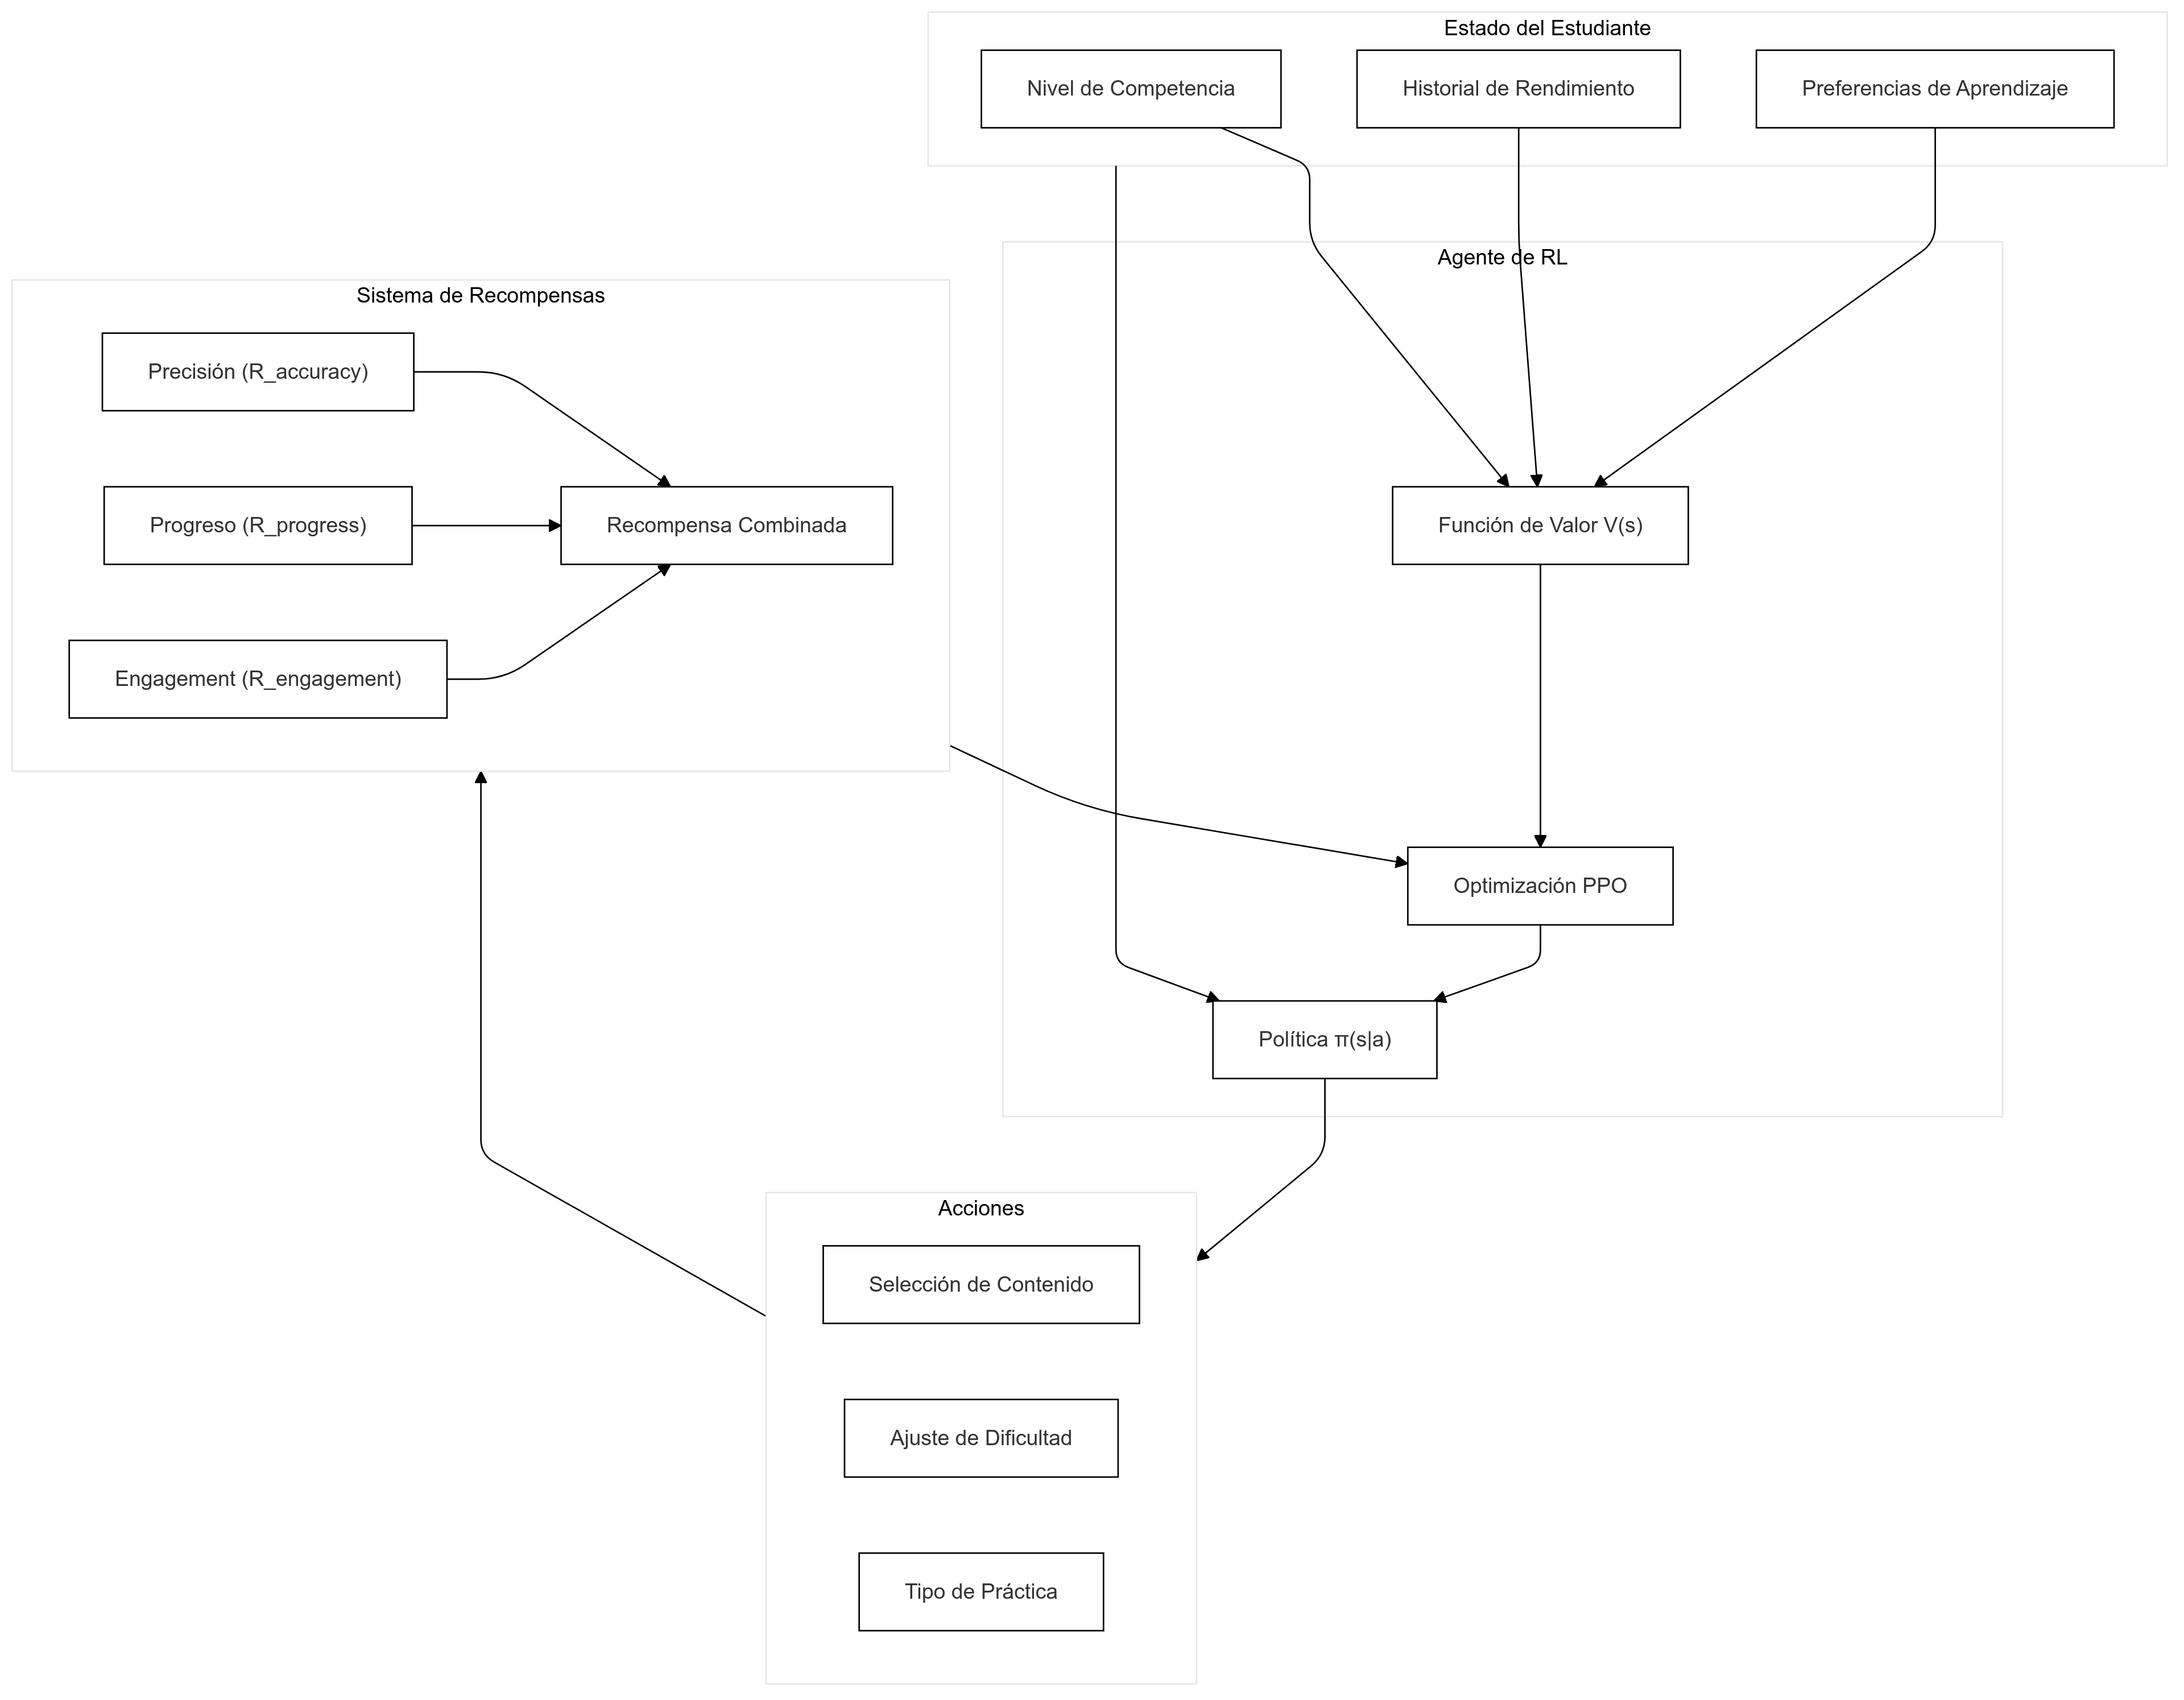
\includegraphics[width=0.8\textwidth]{figuras/rl-flow.png}
\end{figure}

\subsection{Algoritmo de Personalización}
\label{algoritmo-personalizacion}

El sistema implementa un algoritmo de \gls{rl} basado en \gls{ppo} \cite{schulman2017proximal} para optimizar las rutas de aprendizaje. El objetivo es maximizar el aprendizaje a largo plazo mientras se mantiene un nivel apropiado de desafío y engagement.

\subsubsection{Formulación del Problema}

El problema se formula como un \gls{mdp} donde:

\begin{itemize}
    \item \textbf{Estado ($s_t$):} Vector que representa el estado actual del estudiante:
    \begin{equation}
        s_t = [c_1, ..., c_n, h_1, ..., h_m, p_1, ..., p_k]
    \end{equation}
    donde $c_i$ son los niveles de competencia en diferentes habilidades, $h_i$ es el historial de rendimiento, y $p_i$ son las preferencias de aprendizaje.

    \item \textbf{Acciones ($a_t$):} Vector de decisiones pedagógicas:
    \begin{equation}
        a_t = [d, t, c]
    \end{equation}
    donde $d$ es el nivel de dificultad, $t$ es el tipo de ejercicio, y $c$ es el contenido específico.

    \item \textbf{Política ($\pi_\theta$):} La política que mapea estados a acciones:
    \begin{equation}
        \pi_\theta(a_t|s_t) = P(a_t|s_t; \theta)
    \end{equation}
\end{itemize}

\subsubsection{Algoritmo PPO}

El algoritmo PPO optimiza la política mediante la siguiente función objetivo:

\begin{equation}
    \label{eq:ppo-objective}
    L^{CLIP}(\theta) = \mathbb{E}_t[\min(r_t(\theta)A_t, \text{clip}(r_t(\theta), 1-\epsilon, 1+\epsilon)A_t)]
\end{equation}

donde:
\begin{itemize}
    \item $r_t(\theta) = \frac{\pi_\theta(a_t|s_t)}{\pi_{\theta_{old}}(a_t|s_t)}$ es el ratio de probabilidades
    \item $A_t$ es la estimación de ventaja
    \item $\epsilon$ es el parámetro de recorte (típicamente 0.2)
\end{itemize}

La actualización de la política se realiza mediante descenso de gradiente:

\begin{equation}
    \theta_{new} = \theta + \alpha \nabla_\theta L^{CLIP}(\theta)
\end{equation}

\subsection{Sistema de Recompensas}
\label{sistema-recompensas}

Se implementa un sistema de recompensas multiobjetivo que considera tres componentes principales:

\begin{equation}
    \label{eq:reward}
    R = w_1R_{accuracy} + w_2R_{progress} + w_3R_{engagement}
\end{equation}

\subsubsection{Componentes de Recompensa}

\begin{itemize}
    \item \textbf{Precisión ($R_{accuracy}$):} Evalúa la corrección de las respuestas:
    \begin{equation}
        R_{accuracy} = \frac{\text{respuestas\_correctas}}{\text{total\_respuestas}} \cdot \gamma
    \end{equation}
    donde $\gamma$ es un factor de dificultad que aumenta la recompensa para ejercicios más desafiantes.

    \item \textbf{Progreso ($R_{progress}$):} Mide el avance en el dominio de habilidades:
    \begin{equation}
        R_{progress} = \sum_{i=1}^n \Delta c_i \cdot \beta_i
    \end{equation}
    donde $\Delta c_i$ es el cambio en el nivel de competencia de la habilidad $i$, y $\beta_i$ es su peso relativo.

    \item \textbf{Engagement ($R_{engagement}$):} Evalúa la participación activa:
    \begin{equation}
        R_{engagement} = \alpha_t t_{session} + \alpha_c c_{completion} + \alpha_i i_{interaction}
    \end{equation}
    donde $t_{session}$ es la duración de la sesión, $c_{completion}$ es la tasa de finalización, y $i_{interaction}$ es la frecuencia de interacción.
\end{itemize}

\subsubsection{Adaptación de Pesos}

Los pesos $w_i$ se ajustan dinámicamente según el perfil del estudiante mediante un algoritmo de adaptación:

\begin{equation}
    w_i^{new} = w_i + \eta(\bar{R}_i - R_{target}) + \lambda\Delta w_i
\end{equation}

donde:
\begin{itemize}
    \item $\eta$ es la tasa de adaptación
    \item $\bar{R}_i$ es la recompensa promedio reciente para el componente $i$
    \item $R_{target}$ es el valor objetivo
    \item $\lambda\Delta w_i$ es un término de momentum para estabilizar los cambios
\end{itemize}

\section{Metodología de Evaluación}
\label{metodologia-evaluacion}

La evaluación del sistema se realiza en dos dimensiones principales: rendimiento técnico y experiencia de usuario. Este enfoque permite valorar tanto la eficiencia técnica del sistema como su utilidad práctica para los usuarios.

\subsection{Evaluación de Rendimiento}
\label{evaluacion-rendimiento}

La evaluación técnica del sistema se centra en dos aspectos principales:

\subsubsection{Métricas del Sistema}

\begin{itemize}
    \item \textbf{Latencia de Respuesta:} Se mide el tiempo de respuesta del sistema en diferentes puntos:
    \begin{itemize}
        \item Tiempo de procesamiento de solicitudes API
        \item Latencia en la generación de respuestas
        \item Tiempo de renderizado en el cliente
    \end{itemize}

    \item \textbf{Uso de Recursos:}
    \begin{itemize}
        \item Consumo de memoria en el cliente
        \item Utilización de CPU/GPU
        \item Eficiencia en el uso de WebGPU
    \end{itemize}
\end{itemize}

\subsubsection{Rendimiento del Procesamiento de Voz}

\begin{itemize}
    \item \textbf{Precisión en Reconocimiento de Voz:}
    \begin{itemize}
        \item Tasa de error en la transcripción
        \item Precisión en diferentes entornos acústicos
        \item Tiempo de procesamiento
    \end{itemize}

    \item \textbf{Calidad de Síntesis de Voz:}
    \begin{itemize}
        \item Naturalidad de la voz generada
        \item Consistencia en la pronunciación
        \item Velocidad de generación
    \end{itemize}
\end{itemize}

\subsection{Evaluación de Usuario}
\label{evaluacion-usuario}

La evaluación de la experiencia de usuario se realiza mediante un proceso continuo que combina análisis cuantitativo y cualitativo.

\subsubsection{Recopilación de Retroalimentación}

\begin{itemize}
    \item \textbf{Encuestas de Usuario:}
    \begin{itemize}
        \item Evaluación de la facilidad de uso
        \item Satisfacción con las funcionalidades
        \item Percepción de la utilidad del sistema
    \end{itemize}

    \item \textbf{Datos Cualitativos:}
    \begin{itemize}
        \item Comentarios y sugerencias de usuarios
        \item Reportes de problemas
        \item Sugerencias de mejora
    \end{itemize}
\end{itemize}

\subsubsection{Análisis de Patrones de Uso}

\begin{itemize}
    \item \textbf{Métricas de Uso:}
    \begin{itemize}
        \item Duración promedio de las sesiones
        \item Frecuencia de uso
        \item Patrones de interacción
    \end{itemize}

    \item \textbf{Análisis de Comportamiento:}
    \begin{itemize}
        \item Funcionalidades más utilizadas
        \item Puntos de abandono
        \item Patrones de navegación
    \end{itemize}
\end{itemize}

\subsection{Análisis de Resultados}

Los resultados de estas evaluaciones se utilizarán para:

\begin{itemize}
    \item Identificar y corregir problemas técnicos
    \item Mejorar la experiencia de usuario
    \item Optimizar el rendimiento del sistema
    \item Guiar el desarrollo de futuras funcionalidades
\end{itemize}